\subsection{PI1: restauración del contexto}
\label{sec:res-pi1}
% PRISMA ítems 19 (resultados individuales) y 20a (características por síntesis)

% Generado por analysis/src/tablas/tablas.py — no editar a mano.
\begin{table}[!tbp]
\centering
\caption{Taxonomía de PI1 y PI2: estudios del Nivel 2 que alcanzan el umbral de validez ($n = 72$). Un estudio puede tener varios códigos, por lo que los porcentajes de un campo pueden sumar más de 100.}
\label{tab:taxo-pi12}
\footnotesize
\begin{tabular}{@{}l r r@{}}
\toprule
Código & Estudios & \% \\
\midrule
\multicolumn{3}{@{}l}{\textit{PI1 · Técnica de restauración del contexto}} \\
\quad Concatenación del historial & 35 & \num{48.6} \\
\quad Reescritura de la pregunta & 12 & \num{16.7} \\
\quad Clasificación del discurso & 2 & \num{2.8} \\
\quad Resolución explícita de referencias & 2 & \num{2.8} \\
\quad No reportado & 25 & \num{34.7} \\
\multicolumn{3}{@{}l}{\textit{PI2 · Representación del estado}} \\
\quad Historial plano & 38 & \num{52.8} \\
\quad SQL previo (edición) & 11 & \num{15.3} \\
\quad Estructura explícita & 10 & \num{13.9} \\
\quad Grafo & 9 & \num{12.5} \\
\quad Memoria externa & 7 & \num{9.7} \\
\quad Ventana deslizante & 5 & \num{6.9} \\
\quad Resumen & 1 & \num{1.4} \\
\quad No reportado & 11 & \num{15.3} \\
\multicolumn{3}{@{}l}{\textit{PI2 · Actualización del estado}} \\
\quad Implícita (neuronal) & 34 & \num{47.2} \\
\quad Reglas deterministas & 16 & \num{22.2} \\
\quad Generativa (LLM) & 12 & \num{16.7} \\
\quad No reportado & 16 & \num{22.2} \\
\multicolumn{3}{@{}l}{\textit{PI2 · Coste del contexto}} \\
\quad Crece con los turnos & 36 & \num{50.0} \\
\quad Acotado & 14 & \num{19.4} \\
\quad No reportado & 22 & \num{30.6} \\
\bottomrule
\end{tabular}
\end{table}


La taxonomía de PI1 se basa en los \nUmbral{} estudios multiturno del Nivel 2 que alcanzan el umbral de validez (\cref{tab:taxo-pi12}). La técnica más frecuente es la concatenación del historial (35 estudios, 48,6~\%), seguida de la reescritura de la pregunta (12 estudios, 16,7~\%). La clasificación del discurso y la resolución explícita de referencias aparecen en 2 estudios cada una (2,8~\%), y 25 estudios (34,7~\%) figuran como «no reportado o no extraído», es decir, la técnica puede faltar en el informe o no haberse capturado en la extracción asistida por IA. Un estudio puede tener más de un código. Entre los insumos del historial, las preguntas previas están presentes en 59 estudios (81,9~\%), el SQL previo en 32 (44,4~\%), las respuestas del sistema en 13 (18,1~\%) y los resultados de ejecución en 3 (4,2~\%); 11 estudios (15,3~\%) no reportan el insumo.
% fuente: PI1.md

Entre los estudios que reescriben la pregunta figuran Rose-SQL~\cite{Zhou2026RoseSQL}, ACT-SQL~\cite{Zhang2023ACTSQL}, CQR-SQL~\cite{Xiao2022CQRSQL}, DIR~\cite{Li2023DIR}, QURG~\cite{Chai2023QURG} y FANDA~\cite{Liu2019FANDA}. CoE-SQL~\cite{Zhang2024CoESQL} y el trabajo de \en{self-play}~\cite{Liu2022Augmenting} concatenan el historial sin reescritura.

Respecto de la pregunta específica, los contrastes dentro del estudio se agrupan en clases distintas para la reescritura y para la concatenación, de modo que la comparación entre ambas es descriptiva y no procede de un mismo estudio. La mediana de la reescritura es de \efReescMed{}~pp (\efReescN{} estudios) y la de la concatenación de \efConcatMed{}~pp (\efConcatN{} estudios); en ambas clases la dirección es positiva en la mayoría de los estudios. El detalle, con la confianza de cada hallazgo, figura en la \cref{sec:res-efectos} (\cref{fig:pi_efectos_componentes} y \cref{tab:efectos}). Las diferencias frente a la línea base propia de los estudios con reescritura se reportan cada una en su \en{benchmark}, métrica e historial, y no se comparan entre sí; por ejemplo, ACT-SQL reporta +18,3~pp en CoSQL con la métrica QM y el historial SOLO\_PREGUNTAS.
% fuente: PI1.md

\subsection{PI2: representación y actualización del estado}
\label{sec:res-pi2}
% PRISMA ítems 19 (resultados individuales) y 20a (características por síntesis)

La base de PI2 son los mismos \nUmbral{} estudios del Nivel 2 (\cref{tab:taxo-pi12}). La representación más frecuente es el historial plano (38 estudios, 52,8~\%). Le siguen el SQL previo como base de edición (11 estudios, 15,3~\%), la estructura explícita (10, 13,9~\%), el grafo (9, 12,5~\%), la memoria externa (7, 9,7~\%), la ventana deslizante (5, 6,9~\%) y el resumen (1, 1,4~\%); 11 estudios (15,3~\%) no reportan la representación. La actualización del estado es implícita y neuronal en 34 estudios (47,2~\%), se basa en reglas deterministas en 16 (22,2~\%) y es generativa con un LLM en 12 (16,7~\%); otros 16 (22,2~\%) no la reportan.
% fuente: PI2.md

En cuanto al coste del contexto, 36 estudios (50,0~\%) crecen con el número de turnos, 14 (19,4~\%) lo acotan y 22 (30,6~\%) no lo reportan. Los trabajos con estructura explícita incluyen a Rose-SQL~\cite{Zhou2026RoseSQL}, el seguimiento de estados con aprendizaje en contexto~\cite{Hu2022InContext}, SemPlan~\cite{Teixeira2026SemPlan} y el modelado de estados de interacción~\cite{Wang2021Tracking}. Los de grafo son IGSQL~\cite{Cai2020IGSQL}, un grafo heterogéneo de interacción~\cite{Yu2021Interactionmodeling} y una red de relaciones híbrida dinámica~\cite{Hui2021Dynamic}. CoE-SQL~\cite{Zhang2024CoESQL} y EditSQL~\cite{Zhang2019EditSQL} editan el SQL previo.
% fuente: PI2.md

Los campos descriptivos del grafo no se reportan en 64 de los 72 estudios. Entre los 8 que sí los reportan, los nodos son elementos del esquema en 8 estudios, tokens de la pregunta en 4 y valores de la base de datos en 2, y el grafo es dinámico en 7 y estático en 1. Los archivos no incluyen el cruce entre tipo de representación y coste del contexto, solo las frecuencias marginales. Los contrastes dentro del estudio de las clases de grafo o estado estructurado (\efGrafoN{} estudios; mediana de \efGrafoMed{}~pp) y de SQL o resultados previos (\efSQLPrevN{} estudios; mediana de \efSQLPrevMed{}~pp) se presentan en la \cref{sec:res-efectos}.
% fuente: PI2.md

\subsection{PI3: vinculación de esquemas e inferencia de \en{joins}}
\label{sec:res-pi3}
% PRISMA ítems 19 (resultados individuales) y 20a (características por síntesis)

Entre los \nUmbral{} estudios del Nivel 2, la técnica de vinculación no se reporta en 22 (30,6~\%). Entre las reportadas predominan la coincidencia de cadenas (15 estudios, 20,8~\%), la ausencia de vinculación explícita (12, 16,7~\%) y el grafo del esquema (12, 16,7~\%); siguen el \en{prompting} de un LLM (10, 13,9~\%), el clasificador entrenado (9, 12,5~\%), la poda del esquema (7, 9,7~\%) y la recuperación por \en{embeddings} (6, 8,3~\%). La inferencia de \en{joins} es implícita en el modelo en 54 estudios (75,0~\%) y no se reporta en 16 (22,2~\%). Solo 2 estudios usan una inferencia no implícita: UniSAr~\cite{Dou2023UniSAr}, con caminos algorítmicos, y PG-GSQL~\cite{Wang2020PGGSQL}, con un grafo de claves foráneas y restricciones. Un total de 10 estudios (13,9~\%) reportan errores de \en{join}.
% fuente: PI3.md

% Generado por analysis/src/tablas/tablas.py — no editar a mano.
\begin{table}[!tbp]
\centering
\caption{Técnicas de PI3 y PI4 por escenario, con ambos brazos restringidos a los estudios cuya contribución central es PI3 o PI4 (misma regla de entrada): multiturno ($n = 34$) y un turno ($n = 268$). Un estudio puede tener varios códigos. Los estudios de un turno se extrajeron de las páginas iniciales (Nivel 1), por lo que la fila «no reportado» no es comparable entre escenarios. \textsuperscript{b}Técnica de un turno no trasladada al multiturno.}
\label{tab:contraste-pi34}
\footnotesize
\setlength{\tabcolsep}{4pt}
\begin{tabular}{@{}l r r@{}}
\toprule
Código & Multiturno & Un turno \\
\midrule
\multicolumn{3}{@{}l}{\textit{PI3 · Vinculación de esquemas}} \\
\quad LLM con \en{prompting} & 9 (\num{26.5}) & 68 (\num{25.4}) \\
\quad Poda del esquema & 7 (\num{20.6}) & 50 (\num{18.7}) \\
\quad Recuperación por \en{embeddings} & 5 (\num{14.7}) & 44 (\num{16.4}) \\
\quad Clasificador entrenado & 6 (\num{17.6}) & 41 (\num{15.3}) \\
\quad Ninguna explícita & 5 (\num{14.7}) & 31 (\num{11.6}) \\
\quad Grafo del esquema & 5 (\num{14.7}) & 27 (\num{10.1}) \\
\quad Coincidencia de cadenas & 8 (\num{23.5}) & 15 (\num{5.6}) \\
\quad No reportado & 8 (\num{23.5}) & 75 (\num{28.0}) \\
\multicolumn{3}{@{}l}{\textit{PI3 · Inferencia de \en{joins}}} \\
\quad Implícita en el modelo & 26 (\num{76.5}) & 55 (\num{20.5}) \\
\quad Grafo de claves foráneas & 1 (\num{2.9}) & 12 (\num{4.5}) \\
\quad Algorítmica (caminos) & 1 (\num{2.9}) & 8 (\num{3.0}) \\
\quad No reportado & 6 (\num{17.6}) & 193 (\num{72.0}) \\
\multicolumn{3}{@{}l}{\textit{PI4 · Mecanismo}} \\
\quad Retroalimentación de ejecución & 8 (\num{23.5}) & 90 (\num{33.6}) \\
\quad Verificador o crítico & 1 (\num{2.9}) & 58 (\num{21.6}) \\
\quad Autodepuración con LLM & 4 (\num{11.8}) & 40 (\num{14.9}) \\
\quad Autoconsistencia (votación)\textsuperscript{b} & 0 (\num{0.0}) & 36 (\num{13.4}) \\
\quad Aclaración con el usuario & 16 (\num{47.1}) & 6 (\num{2.2}) \\
\quad Abstención & 3 (\num{8.8}) & 8 (\num{3.0}) \\
\quad Reparación simbólica\textsuperscript{b} & 0 (\num{0.0}) & 6 (\num{2.2}) \\
\quad No reportado & 12 (\num{35.3}) & 105 (\num{39.2}) \\
\multicolumn{3}{@{}l}{\textit{PI4 · Señal}} \\
\quad Resultado de la ejecución & 7 (\num{20.6}) & 91 (\num{34.0}) \\
\quad Error del SGBD & 7 (\num{20.6}) & 56 (\num{20.9}) \\
\quad Juicio de un LLM & 3 (\num{8.8}) & 48 (\num{17.9}) \\
\quad Usuario & 15 (\num{44.1}) & 8 (\num{3.0}) \\
\quad Resultado vacío & 1 (\num{2.9}) & 7 (\num{2.6}) \\
\quad No reportado & 11 (\num{32.4}) & 120 (\num{44.8}) \\
\bottomrule
\end{tabular}
\end{table}


La \cref{tab:contraste-pi34} contrasta las frecuencias de cada código entre los \nCentralMT{} estudios multiturno y los \nCentralUT{} de un turno cuya contribución central es PI3 o PI4, con la misma regla de entrada en ambos brazos y sin aplicar el umbral de validez; por ello los recuentos multiturno difieren de los de la taxonomía anterior (p.\,ej., \nctLinkLlmPromptingMT{} frente a 10 estudios con \en{prompting} de un LLM). Los estudios de un turno se extrajeron de las páginas iniciales (Nivel 1), de modo que las filas «no reportado o no extraído» no son comparables entre escenarios. Las frecuencias del \en{prompting} de un LLM, la poda y la recuperación por \en{embeddings} son similares en ambos brazos (\ctLinkLlmPromptingMT{} y \ctLinkLlmPromptingUT{}~\%; \ctLinkPodaEsquemaMT{} y \ctLinkPodaEsquemaUT{}~\%; \ctLinkEmbeddingsRecuperacionMT{} y \ctLinkEmbeddingsRecuperacionUT{}~\%). La coincidencia de cadenas representa el \ctLinkCoincidenciaCadenasMT{}~\% de los estudios multiturno y el \ctLinkCoincidenciaCadenasUT{}~\% de los de un turno, y el grafo del esquema el \ctLinkGrafoEsquemaMT{}~\% frente al \ctLinkGrafoEsquemaUT{}~\%. La inferencia implícita de \en{joins} figura en el \ctJoinsImplicitaModeloMT{}~\% de los estudios multiturno y el \ctJoinsImplicitaModeloUT{}~\% de los de un turno, pero la inferencia de \en{joins} figura como no reportada o no extraída en el \ctJoinsNrUT{}~\% de los de un turno frente al \ctJoinsNrMT{}~\% de los multiturno, de modo que esta comparación no es válida. La comparación es de frecuencias, no de resultados.
% fuente: pi34_tecnicas_central.csv, PI3.md

Como análisis exploratorio, la \cref{fig:bib_coocurrencia_tecnicas} (\cref{app:figuras}) muestra las combinaciones de técnicas de PI3 y PI4 en un mismo estudio. En multiturno, la aclaración con el usuario se combina con la retroalimentación de ejecución, con el \en{prompting} de un LLM y con la coincidencia de cadenas en 6 estudios cada una. En un turno, la retroalimentación de ejecución coincide con el \en{prompting} de un LLM en 31 estudios y este con la autoconsistencia en 19. La mediana de los contrastes dentro del estudio de la vinculación de esquemas es de \efVincMed{}~pp (\efVincN{} estudios); su detalle se presenta en la \cref{sec:res-efectos}.
% fuente: bib_coocurrencia_multiturno.csv, bib_coocurrencia_un_turno.csv, PI3.md

\subsection{PI4: retroalimentación de ejecución y autocorrección}
\label{sec:res-pi4}
% PRISMA ítems 19 (resultados individuales) y 20a (características por síntesis)

En los \nUmbral{} estudios del Nivel 2, el mecanismo de autocorrección no se reporta en 46 (63,9~\%) y la señal en 47 (65,3~\%). Entre los reportados, la aclaración con el usuario aparece en 18 estudios (25,0~\%), la retroalimentación de ejecución y errores en 10 (13,9~\%), la abstención y la autodepuración con un LLM en 4 cada una (5,6~\%), el verificador o crítico en 2 (2,8~\%) y la reparación simbólica en 1 (1,4~\%). Las señales son el usuario (16 estudios, 22,2~\%), el resultado de la ejecución (9, 12,5~\%), el error del SGBD (9, 12,5~\%), el juicio de un LLM (3, 4,2~\%) y el resultado vacío (2, 2,8~\%). El mecanismo se aplica al escenario multiturno en 30 estudios (41,7~\%) y no en 42 (58,3~\%). Ejemplos son la aclaración en un analizador interactivo~\cite{Elgohary2020Speak}, la retroalimentación de ejecución con aprendizaje a partir de errores~\cite{Zhai2024Learn}, HarnessSQL~\cite{Yang2026HarnessSQL}, la reparación simbólica de PICARD~\cite{Scholak2021PICARD} y un verificador conversacional~\cite{HariKrishnanParthasarathi2023Conversational}.
% fuente: PI4.md

El contraste con un turno aparece en la \cref{tab:contraste-pi34}, con la misma base restringida a PI3/PI4 centrales que en PI3. La retroalimentación de ejecución está en el \ctMecEjecucionFeedbackErroresMT{}~\% de los estudios multiturno y el \ctMecEjecucionFeedbackErroresUT{}~\% de los de un turno, una diferencia menor que la del contraste previo sin restringir; el verificador o crítico, en el \ctMecVerificadorCriticoMT{}~\% frente al \ctMecVerificadorCriticoUT{}~\%, y la autodepuración con un LLM, en el \ctMecAutodepuracionLlmMT{}~\% frente al \ctMecAutodepuracionLlmUT{}~\%. La aclaración con el usuario ocurre en el \ctMecAclaracionUsuarioMT{}~\% de los estudios multiturno y el \ctMecAclaracionUsuarioUT{}~\% de los de un turno, y la señal de usuario en el \ctSenalUsuarioMT{}~\% frente al \ctSenalUsuarioUT{}~\%, de modo que ambas siguen siendo mucho más frecuentes en multiturno. La autoconsistencia por votación y la reparación simbólica no figuran en ningún estudio multiturno de la tabla y aparecen en \nctMecAutoconsistenciaVotacionUT{} (\ctMecAutoconsistenciaVotacionUT{}~\%) y \nctMecReparacionSimbolicaUT{} (\ctMecReparacionSimbolicaUT{}~\%) de un turno, respectivamente. Las medianas de los contrastes dentro del estudio son de \efAutocorrMed{}~pp para la autocorrección por ejecución (\efAutocorrN{} estudios) y de \efAclarMed{}~pp para la aclaración (\efAclarN{} estudios), con los detalles y la confianza en la \cref{sec:res-efectos}.
% fuente: pi34_tecnicas_central.csv, PI4.md

\subsection{PI5: \en{benchmarks}, métricas y degradación por turno}
\label{sec:res-pi5}
% PRISMA ítems 19 (resultados individuales) y 20c (causas de heterogeneidad)

% Generado por analysis/src/tablas/tablas.py — no editar a mano.
\begin{table*}[!tbp]
\centering
\caption{PI5: historial usado en la evaluación y degradación por turno, estudios del Nivel 2 que alcanzan el umbral de validez ($n = 72$). La pendiente es la mediana por estrato; los estratos no se combinan.}
\label{tab:pi5}
\footnotesize
\begin{tabular}{@{}l r r r r@{}}
\toprule
Estrato o práctica & Estudios (\%) & Est. con curva & Curvas & Pendiente (pp/turno) \\
\midrule
\multicolumn{5}{@{}l}{\textit{Historial usado en la evaluación}} \\
\quad Predicho & 31 (\num{43.1}) & 5 & 6 & \num{-7.0} \\
\quad Solo preguntas & 19 (\num{26.4}) & 6 & 8 & \num{-11.0} \\
\quad De referencia (\en{gold}) & 5 (\num{6.9}) & --- & --- & --- \\
\quad No reportado & 20 (\num{27.8}) & --- & --- & --- \\
\multicolumn{5}{@{}l}{\textit{Prácticas de reporte (estudios que sí las reportan)}} \\
\quad Degradación por turno & 38 (\num{52.8}) & & & \\
\quad Errores de \en{join} & 10 (\num{13.9}) & & & \\
\quad Contaminación del \en{benchmark} & 7 (\num{9.7}) & & & \\
\bottomrule
\end{tabular}
\end{table*}


Los \nUmbral{} estudios del Nivel 2 con validez suficiente usan sobre todo \en{benchmarks} multiturno conversacionales (50 estudios), seguidos de \en{benchmarks} estándar de un turno (18), interactivos o de aclaración (11), variantes de un turno (7), de diálogo orientado a tareas (5), de datos propios o industriales (3) y de QA conversacional o tabular híbrida (3). Entre ellos se cuentan SParC~\cite{Yu2019SParC}, CoSQL~\cite{Yu2019CoSQL} y CHASE~\cite{Guo2021Chase}, además de Spider~\cite{Yu2018Spider} y BIRD~\cite{Li2023BIRD} en su uso de un turno. Las métricas más empleadas son la ejecución por pregunta (34 estudios), la coincidencia por interacción (31) y la coincidencia por pregunta (30), seguidas de la coincidencia exacta o lógica (21) y la ejecución por interacción (9). Un estudio puede aparecer en varias familias. Las categorías \texttt{OTRA} se consolidaron en las familias anteriores.
% fuente: PI5.md

% Generado por analysis/src/tablas/figuras_tex.py — no editar a mano.
\begin{figure*}[!tbp]
\centering
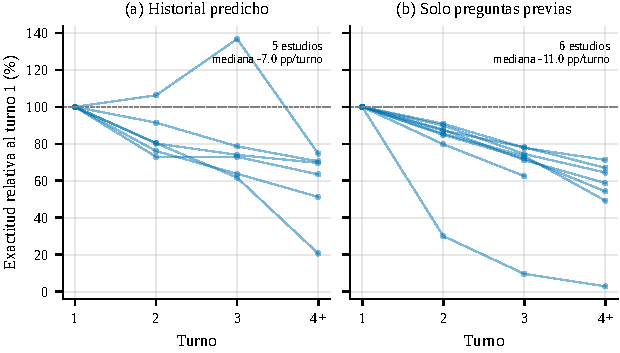
\includegraphics[width=4.14in,height=0.85\textheight,keepaspectratio]{pi5_degradacion}
\caption{Degradación de la exactitud a lo largo de los turnos (sistema propuesto, normalizada al turno 1; turnos $\geq$ 4 agrupados en «4+»), separada por el tipo de historial usado en la evaluación: (a) historial predicho; (b) solo preguntas previas. Valores por turno extraídos de las tablas de cada estudio y verificados en la página citada. Sin curvas con al menos tres turnos para: historial gold, no reportado. Los grupos de turno contienen preguntas distintas, por lo que la pendiente mezcla profundidad y dificultad; las pendientes no se agrupan entre estratos.}
\label{fig:pi5_degradacion}
\end{figure*}


El tipo de historial usado en la evaluación (\cref{tab:pi5}) es predicho en 31 estudios (43,1~\%), solo preguntas en 19 (26,4~\%), de referencia (\en{gold}) en 5 (6,9~\%) y no reportado o no extraído en 20 (27,8~\%). Un total de 38 estudios (52,8~\%) reportan degradación por turno, 10 (13,9~\%) errores de \en{join} y 7 (9,7~\%) discuten la contaminación del \en{benchmark}. En la muestra independiente de la autora, el historial coincidió en 3 de 5 estudios (60,0~\%); las discrepancias correspondieron a SUQL~\cite{Liu2024SUQL} y DIR~\cite{Li2023DIR}, y la primera se corrigió a SOLO\_PREGUNTAS. La estratificación de PI5 depende, por tanto, de una codificación verificada de forma independiente en 3 de 5 estudios de la muestra.
% fuente: PI5.md

La \cref{fig:pi5_degradacion} presenta la degradación por turno, con los estratos separados y sin agruparlos. En el estrato predicho hay 6 curvas de 5 estudios, con una pendiente mediana de $-7{,}0$~pp por turno (rango de \degPredMin{} a \degPredMax{}~pp por turno). En el estrato de solo preguntas hay 8 curvas de 6 estudios, con una mediana de $-11{,}0$~pp por turno (rango de \degSoloMin{} a \degSoloMax{}~pp por turno). Ninguna curva con al menos tres turnos corresponde al historial de referencia ni al no reportado. Todas las pendientes individuales son negativas en ambos estratos; por ejemplo, la de IGSQL~\cite{Cai2020IGSQL} en SParC es de $-16{,}95$~pp por turno (historial predicho) y la de QURG~\cite{Chai2023QURG} en SParC de $-10{,}62$~pp (solo preguntas). Los valores relativos superiores al 100~\% de la figura indican que algunos grupos de turnos posteriores puntúan más que el turno 1. Los grupos de turno contienen preguntas distintas, por lo que la pendiente mezcla la profundidad del turno con la dificultad de las preguntas, y las comparaciones entre filas son descriptivas.
% fuente: PI5.md, revision_4f.json (A9_degradacion)

\subsection{Sesgos de notificación y análisis de sensibilidad complementarios}
\label{sec:res-sesgos}
% PRISMA ítems 20d (sensibilidad) y 21 (sesgos de notificación)

Varios campos de la extracción figuran como no reportados o no extraídos en una parte amplia de los estudios del Nivel 2: la técnica de restauración del contexto en 25 de 72 (34,7~\%), el mecanismo de autocorrección en 46 de 72, el historial de la evaluación en 20 de 72 y los campos descriptivos del grafo en 64 de 72. Los contrastes con dirección negativa son escasos: se registra un estudio en la reescritura de la pregunta, uno en SQL o resultados previos y uno en la aclaración, entre otros.
% fuente: PI1.md, PI2.md, PI4.md, PI5.md

La reincorporación de los \nBajoUmbral{} estudios bajo el umbral de validez no modificó las medianas de PI1 ni de PI2. En PI3 la mediana de otros componentes pasó de \efPItresOtrosMed{} a \efPItresOtrosMedTodos{}~pp y en PI4 la de otros componentes de \efPIcuatroOtrosMed{} a \efPIcuatroOtrosMedTodos{}~pp, y la clase de autocorrección por ejecución pasó de \efAutocorrN{} a \efAutocorrNTodos{} estudios, con una mediana de \efAutocorrMedTodos{}~pp. Al excluir los preprints, la mediana de SQL o resultados previos pasó de \efSQLPrevMed{} a \efSQLPrevMedSinPre{}~pp (\efSQLPrevNSinPre{} estudios) y la de vinculación de esquemas de \efVincMed{} a \efVincMedSinPre{}~pp (\efVincNSinPre{} estudios); las demás medianas variaron poco o nada. La clase de aclaración no figura en el análisis sin preprints. Las sensibilidades de D4 se presentan en la \cref{sec:res-d4}.
% fuente: PI1.md, PI3.md, PI4.md, PI2.md

Los informes no recuperados corresponden a 148 de señal de un turno y 43 de señal multiturno. Con el supuesto extremo de que todos cuentan en el denominador y los de señal multiturno también en el numerador, D4 es de \DcuatroCotaK/\DcuatroCotaN{} (\DcuatroCotaPct~\%; IC 95~\% de \DcuatroCotaICinf{} a \DcuatroCotaICsup~\%); la estimación probabilística da D4 $\approx$ \DcuatroProbPct~\%.
% fuente: PI0.md, revision_4f.json (A7_cota_probabilistica)
%%%% END
